\documentclass[12pt]{article}
\usepackage{natbib}
\usepackage{graphicx}
\usepackage{float}
\usepackage[hyphenbreaks]{breakurl}
\usepackage[hyphens]{url}



%Gummi|065|=)
\title{\textbf{ID2203 Project}}
\author{Max Meldrum\\
	Vaikunth Srinivasan A}
\date{}
\begin{document}

\maketitle

\section{Introduction}
In this project, we will implemented a distributed in memory key-value store with linearizable operation semantics. We take advantage of the Kompics \cite{DBLP:conf/p2p/AradDH09} programming model and utilise the Kompics Scala DSL. We were given a lot of freedom when it came to the design of the system, as long as we satisfied linearizability.
\section{Infrastructure}
In this section, we describe how our system is designed.

\subsection{Overview}

The key-value store is portioned based on the key-space with each partition responsible for a particular key range. The partitions constitute a replication group i.e., each partition consists of a primary and its replicas. The replication groups are responsible for handling client requests and providing linearizable operation semantics.


\begin{figure}[H]
  \centering
  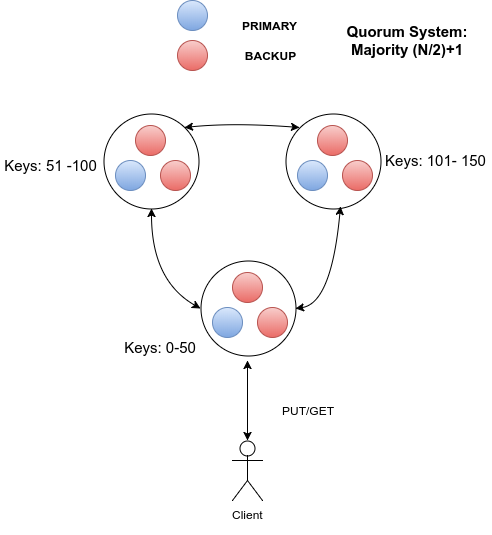
\includegraphics[scale=0.6,clip]{img/architecture}
  \caption[Caption for LOF]{System architecture}  
  \label{fig:picture}
\end{figure}

\subsection{Partitioning}
As one of the requirements was that the system should e able to support a partitioned key-space, we have opted to go for range-partitioned integers. These partitions are distributed over the available nodes. Each partition is considered to be a replication group and we use passive replication where each of these groups consist of one primary and multiple backups. The replication within a group is done with respect to a specific replication degree.

\subsection{System Model}
We decided to go for the fail-silent model, where we assume our environment to be asynchronous. To ensure consistency across all replicas in a certain replication group, we use a primary-backup scheme and implement an Atomic Broadcast protocol that is heavily inspired by Zab \cite{Junqueira:2011:ZHB:2056308.2056409} which ZooKeeper \cite{Hunt:2010:ZWC:1855840.1855851} relies on.

\subsubsection{Assumptions}
We are assuming that all our network based components have access to a perfect-link abstraction.

\section{Replication Protocol}

\subsection{Atomic Broadcast}
Zab, which is the algorithm behind ZooKeeper, is a crash-recovery atomic broadcast algorithm. A primary server handles client requests and broadcast state changes to the rest of the backups. The delivery order of state updates is crucial. This order is often referred as Primary Order \cite{Junqueira:2011:ZHB:2056308.2056409}. Zab consists of 3 phases. However, as we are not implementing our kv-store in a crash-recovery model, we skip the synchronising phase and only implement Leader Activation and Active Messaging \cite{zk-internals}.
\newline{}\newline{}
In this report, we will put more focus on describing on how the broadcast phase works and not so much on Leader Activation. Zab assumes all communication channels are FIFO, so that everything is done in order. This was not an issue for us as the channels in Kompics provide FIFO semantics. The Active Messaging in Zab is very similar to a classic two-phase commit.  Once a primary has received a client request, it broadcasts out proposals that includes its monotonically unique proposal id. Replica’s that receive proposals return with an acknowledgement (ACK). As soon as the primary has received a majority of ACKs for a given proposal, it will issue a commit to itself and its backups. This whole process can be seen in figure 2 down below.


\begin{figure}[H]
  \centering
  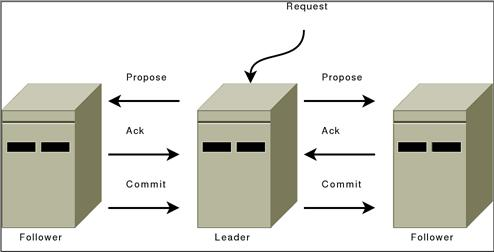
\includegraphics[scale=0.90]{img/2pc.jpg}
  \caption[Caption for LOF]{ZooKeeper messaging \protect \cite{zk-internals}}  
  \label{fig:picture}
\end{figure}


\subsection{Failure Detection}
As we are in the fail-silent model, we do not rely on a perfect failure detector or an eventually perfect failure detector. We utilise the Zab approach, where the primary periodically checks if it has a majority of replicas connected to it. This means that backups frequently send heartbeats to the primary. If a primary notices that it no longer has a majority of followers connected, it enters an election phase. What if backup’s are isolated and cannot connect with anyone? The solution to this is that backup’s also receives heartbeats from the primary. If a backup stops hearing from a primary, it will enter into an election phase and attempt to elect a new primary.



\section{Testing}

\subsection{Operations}
\subsection{Linearizability}


\section{Conclusion}

\bibliography{references}
\bibliographystyle{unsrt}


\end{document}
